\chapter{Constraint Programming}
\label{sec:CP}

\cite{CPforScheduling} definieren {\bf Constraint Programming} (deutsch: Bedingungsprogrammierung, Constraintsprogrammierung, {\bf CP}) als eine Methode zur Formulierung und Lösung eines diskreten Bedingungserfüllungs- oder Bedingungsoptimierungsproblems durch systimatische Anwendung deduktiver Folgerungen, um den Suchraum zu minimieren. CP ist eine Erweiterung der logischen Programmierung, da sie erlaubt,  verschiedene mächtige Suchalgorithmen zu benutzt und sie für jedes spezifisches Problem entsprechend anzupassen. Das macht diese Programmierparadigma sehr flexibel, fordert aber eine bestimmte Erfahrung in der deklarativen logischen Programmierung und in der Entwicklung von Suchalgorithmen \citep[vgl][]{CPforScheduling}.

In diesem Kapitel definieren wir die Hauptbegriffe aus der Theorie der CP, stellen allgemeinen CP Programmierungsgerüst vor und am Ende machen einen Vergleich zwischen CP und gemischter ganzzahliger Optimierung (Mixed-Integer Programming, {\bf MIP}).

\section{Constraint Satisfication Problem}

{\bf Constraint Satisfication Problem} (deutsch: Bedingungserfüllungsproblem, {\bf CSP}) ist ein Problem der Zuweisung gegebenen Variablen die Werte aus der gegebenen Definitionsbereichen, so dass alle Bedingungen an die Variable erfüllt sind \citep[vgl][]{CSP}. Formeller:\\
Gegeben seien die Menge $X= \{ x_1,x_2,\dots, x_n\}$ diskreten Variablen zusammen mit ihren endlichen Definitionsbereichen $\{ D_1,D_2,,\dots D_n\}$ und die Menge der Bedingungen $C_{ijk\dots}$ zwischen den Variablen $x_i, x_j, x_k, \dots$, die die mögliche Werte der Variablen zusätzlich einschränken.
%\footnote{Wir betrachten den Fall, wenn die Definitionsbereiche der Variablen eine Folge konsekutiven ganzen Zahlen darstellen}

Im allgemeinen können die Variable von verschiedenen Typen sein (ganzzahlig, boolean, symbolisch, Mengen). Dafür gibt es verschiedene Typen der Bedingungen:
\begin{itemize}
	\setlength{\itemsep}{0pt}
	\item mathematische (Fertigstellungszeit = Startzeit + Bearbeitungszeit),
	\item disjunktive (Jobs $J_1$ und $J_2$ müssen an verschiedenen Maschinen abgearbeitet werden),
	\item relational (die Maschine $I$ kann höchstens vier Jobs abarbeiten),
	\item explizite (die Arbeiten $J_1$, $J_2$ und $J_5$ können nur auf der Maschine abgearbeitet werden).
\end{itemize}
Ein CSP besitzt eine {\bf (zulässige) Lösung}, wenn es eine Zuweisung der Werten aus der  Definitionsbereich zu jeder Variable existiert, sodass alle Bedingungen erfüllt sind. Abhängig von der Aufgabe kann man sich für eine oder für alle zulässige Losungen interessieren.

\subsection{Allgemeiner Algorithmus zur Lösung des Constraint Satisfaction Problems}

Auf der Abbildung \ref{fig:CSPalgorithm} (\cite{CPforScheduling}) ist der allgemeine Algorithmus zur Lösung eines CSP dargestellt. 

Man beginnt mit der Definition der Variablen, ihrer Definitionsbereichen und Bedingungen %Constraints
(siehe Block $1$).

Block $2$ repräsentiert den Prozess der {\bf Bedingungsfortpflanzung} (engl. {\bf constraint propagation}) und der {\bf Reduktion von Definitionsbereichen} (engl. {\bf domain reduction}).  Das bedeutet, dass aus den vorhandenen Bedingungen durch die Anwendung der auf der Logik basierten Filteralgorithmen neue Bedingungen abgeleitet werden, die systematisch die Definitionsbereiche von Variablen reduzieren oder zu einem Widerspruch führen.

Nach der Reduktion von Definitionsbereichen bestehen zwei Möglichkeiten (Block $3$): entweder ist eine Lösung der Problem gefunden oder nicht. Im ersten Fall terminiert der Algorithmus. Im zweiten wird geprüft, ob das Problem widersprüchlich ist (Block $4$).

Wenn das Problem nicht widersprüchlich ist (siehe Pfeile $6$), man wendet einen Suchverfahren für {\bf die Verzweigung} (engl. {\bf branching}) an. Das Ziel der Verzweigung ist die Aufteilung des ursprüngliches Problems in eine Menge von gegenseitig ausschließenden Teilproblemen, die aber zusammen die Lösung des Problems vollständig beschreiben. Es wird so genannten Entscheidungsbaum gebildet.

Jeder Zweig repräsentiert das Hinzufügen der zusätzlichen Bedingungen, die das Problem einschränken. Bei der Verzweigung wird einen der Zweige gewählt und man beginnt erneut mit der Bedingungsfortpflanzung (Block $2$) das Teilproblem zu lösen.

Wenn das Problem sich im Block $4$ als widersprüchlich erwiesen hat, wird im Block $5$ geprüft, ob alle Teilprobleme untersucht wurden. Falls nicht (Block $7$), geht der Algorithmus im Entscheidungsbaum eine Stufe höher, wählt ein anderes Teilproblem aus und versucht es zu lösen. Sonst ist die Widersprüchlichkeit des Problems nachgewiesen und der Algorithmus terminiert.

\begin{figure}[h]
	\centering
	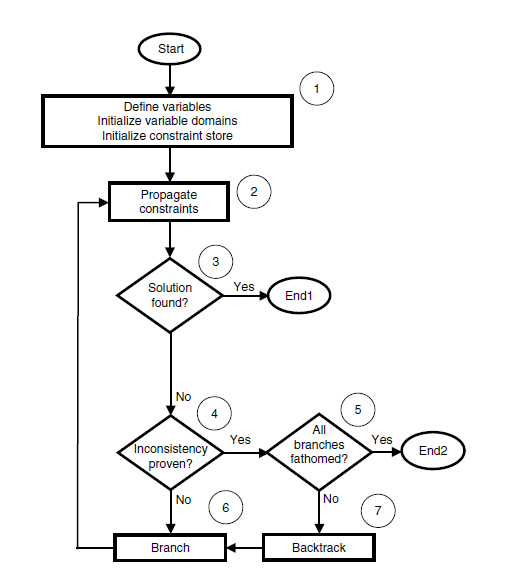
\includegraphics[scale=0.9]{fig/CSPalgorithm.png}
	\caption{Allgemeiner Algorithmus für das Constraint Satisfaction Problem }
	\label{fig:CSPalgorithm}
\end{figure}

\FloatBarrier

\subsection{Bedingungsfortpflanzung (constraint propagation)}

Das Verfahren der Bedingungsfortpflanzung prüft die Widerspruchsfreiheit der im Problem vorhandenen Bedingungen, um die neue ableiten zu können (eng. {\bf arc consistency checking}).

Hier geht man davon aus, dass die Bedingungen zwischen der Variablen eines CSP immer nur zwei Variablen beeinflussen. In diesem Fall kann CSP als ein Bedingungsgraph dargestellt werden. Variablen des CSP bilden die Menge der Knoten des Graphen. Die Knoten sind adjazent, wenn es eine Bedingung gibt, die die entsprechende Variable verbindet \citep[vgl.][]{CSP}.

Sei eine Bedingung $C_{ij}$ zwischen den Variablen $x_i$ und $x_j$ gegeben. Der Bogen $(x_i,x_j)$ heißt widerspruchsfrei (eng. {\bf consistent}), wenn für jeden Wert $a\in D_i$ ein Wert $b\in D_j$ existiert, sodass die Zuweisungen $x_i=a$ und $x_j=b$ die Bedingung $C_{ij}$ erfüllen (\cite{CSP}).

\newpage

\begin{wrapfigure}[10]{l}{0.5\textwidth}
	\vspace{-10pt}
	\vbox{
		\centering
		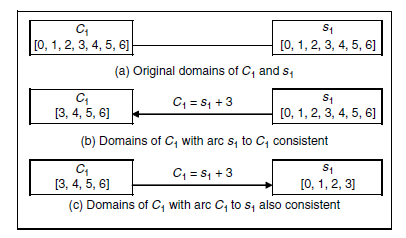
\includegraphics[scale=0.7]{fig/ConstraintPropagation1.png}
	}
	\caption{Reduktion des Suchraums mithilfe der Widerspruchsfreiheit eines Bogens}
	\label{fig:ConstraintPropagation1}
\end{wrapfigure}

Alle Werte $a\in D_i$, für die dies nicht gilt, können aus der Definitionsbereich $D_i$ der Variable $x_i$ gelöscht werden, da sie keine zulässige Lösung bilden können. Das Löschen von solcher Werte macht den Bogen widerspruchsfrei. Ein einfaches Beispiel der Bogenwiderspruchsfreiheit ist auf der Abbildung \ref{fig:ConstraintPropagation1} (\cite{CPforScheduling}) dargestellt.

\FloatBarrier

Offensichtlich, wenn alle Bogen widerspruchsfrei gemacht wurden, ist der Suchraum des Problems kleiner geworden (engl. {\bf domain reduction}). Nach der Reduktion des Suchraums soll das Suchen nach der Lösung einfacher werden.

Zu bemerken ist, dass die Bedingungsfortpflanzung die Informationen über der Definitionsbereichen der Variablen nicht nur innerhalb einer Bedingung benutzen kann, sondern auch zwischen mehreren Bedingungen. Dazu das Beispiel auf der Abbildung \ref{fig:ConstraintPropagation2} (\cite{CPforScheduling}). Das führt zu der so genannten Reduktion des Suchraums zwischen der Bedingungen (eng. {\bf between-constraint domain reduction}).

\begin{figure}[h]
	\centering
	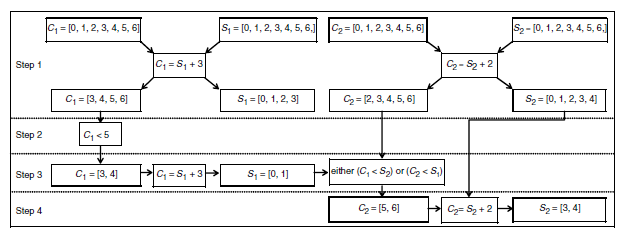
\includegraphics[scale=0.8]{fig/ConstraintPropagation2.png}
	\caption{Reduktion des Suchraums mithilfe der Widerspruchsfreiheit mehreren Bogen}
	\label{fig:ConstraintPropagation2}
\end{figure}

\subsection{Branching}

Typischerweise es wird Backtracking- Verfahren fürs Branching (siehe Block $6$ auf der Abbildung \ref{fig:CSPalgorithm}) verwendet, der aber oft ineffizient ist. Deswegen werden auch andere Verfahren wie Forward checking oder MAC (von engl. maintaining arc consistency) verwendet \citep[vgl.][]{CSP}. Ihre Vorteil sind, dass sie so genannte lookahead Verfahren sind. D.h. jeder Zweig beeinflusst die Definitionsbereichen aller Variablen und nicht nur derjenigen, die im Suchbaum früher betrachtet wurden.

Auf jeden Fall bleibt die Frage offen, wo als erstes verzweigt werden muss. An dieser Stelle werden verschieden Heuristiken verwendet, wie z.B. es wird als erstes in Variable mit der kleinsten Definitionsbereich verzweigt.

Nachdem der Wahl der Variable getroffen wurde, wird ein neuer Zweig im Suchbaum gebildet, indem man dieser Variable einen Wert aus ihrer Definitionsbereich zuweist. Hier wird wiederum heuristisch entschieden, welchen Werte diese Variable annehmen soll. Häufige Vorgehensweise ist den kleinsten Wert aus der Definitionsbereich der Variable zu nehmen.

In allgemeinen kann die Verzweigung auf verschiedene weise verlaufen: es kann einen Wert zu einer Variable, mehrere Werte zu einer Variable oder mehrere Werte zu mehreren Variablen zugewiesen werden.

\section{Constraint Optimierungsproblem}
Klassisches CSP kann einfach zur {\bf Constraint Optimierungsproblem} (engl. Constraint Optimization Problem, {\bf COP}) erweitert werden. 

Angenommen unseres COP hat eine Zielfunktion $Z$, die minimiert werden soll. Wenn wir das Problem ohne Zielfunktion betrachten, ist es ein CSP und seine Lösung können wir mit Hilfe vom Algorithmus auf der Abbildung \ref{fig:CSPalgorithm} finden. Sobald erste Lösung von SCP gefunden wurde, berechnen wir den Wert der Zielfunktion ($Z'$) und fügen die Bedingung $Z<Z'$ zum Problem hinzu. Als Ergebnis bekommen wir ein neues CSP, suchen nach seine Lösung und so weiter, bis es zu einem Widerspruch gekommen ist und alle Zweige im Suchbaum untersucht wurden. Die zuletzt gefundene zulässige Lösung  ist Lösung vom COP.

\section{Vorteile von Constraint Programmierung}

In diesem Abschnitt möchten wir die Vorteilen der Constraint Programmierung vorstellen, die diese Programmierparadigma attraktiv zum Lösen der Scheduling-Aufgaben  machen.

\subsection {Indexierung der Variable}
Analog zu den Programmiersprachen ermöglicht CP die Benutzung einer Variablen als Indizes der anderen Variablen, was normalerweise Anzahl der  Entscheidungsvariablen reduziert.

Die CP-Formulierungen sind deswegen kompakt und intuitiv verständlich.

Als Beispiel betrachten wir ein Einzelmaschine-Batch-Sequenzierung-Problem mit den Reihenfolgenabhängigen Rüstzeiten aus \cite{Jordan}. Die Zielfunktion ist die Minimierung von Rüstkosten und Verfrühungstrafen bei den gegeben Rüstzeiten der adjazenten Jobs in der Reihenfolge.

In IP\footnote{engl. Integer Programming, de. Ganzzahlige Programmierung} werden binäre Variablen $y[i,j]$ benutzt, um zu zeigen, ob Job $i$ sofort nach dem Job $j$ abgearbeitet wird. Falls es insgesamt $n$ Jobs gibt, dann braucht man $n(n-1)$ binäre Variablen $y$, um alle mögliche Reihenfolge der Jobsbearbeitung zu definieren. Sei $cost[i,j]$ der Preis der Bearbeitung des Jobs $i$ sofort nach dem Job $j$. Dann der gesamt Preis der Jobsreihenfolge ist definiert durch $\sum_{i,j,i\not =  j} {cost[i,j]y[i,j]}$.

Um dieses Problem in CP formulieren zu können, definiert man die Entscheidungsvariablen $job[k]$, deren Wert dem Index desjenigen Jobs gleich ist, der als $k$-ter in der Reihenfolge abgearbeitet wird. Es ist klar, dass es insgesamt $n$ solcher Variable gibt. Mit diesen Variablen is der gesamt Preis der Jobsreihenfolge gleich $\sum_{k>1} {cost[job[k-1],job[k]]}$.

Somit ist die Anzahl der Variablen des Problems von $n(n-1)$ auf $n$ reduziert.

\subsection{Nebenbedingungen}

Die CP verfügt über eine Menge der Operationen, die ermöglichen, viele Bedingungen einfach zu formulieren. Wir beschreiben hier einige Bedingungen aus der Scheduling-Theorie, die sich sehr einfach in CP, aber nicht in IP formulieren lassen (siehe Tabelle \ref{table:ConstraintsCPvsIP}).

Angenommen wir haben ein Problem mit zwei Maschinen. Die Variable $MaschineA$ und $MaschineB$ können im ersten Fall Wert $0$ haben, falls es keinen Job gibt, der auf der Maschine abgearbeitet werden muss, oder $1$ sonst. Wir suchen nach solcher Zuordnung der Jobs zu diesen Maschinen, dass nur eine Maschine im Betrieb sein kann. 

\vspace{5pt}
\begin{table}[htb]
\begin{tabular}{c||c} 
	\hline
	CP & IP \\
	\hline
	\hline
	\multicolumn{2}{c}{Fall $1$: Ungleichungen mit den binären Variablen} \\
	\hline
	$MaschineA\not =MaschineB$ & $MaschineA+MaschineB = 1$ \\
	\hline
	\multicolumn{2}{c}{Fall $2$: Ungleichungen mit den ganzzahligen Variablen} \\
	\hline
	$MaschineA\not =MaschineB$ & $(MaschineA - MaschineB - \epsilon +\sigma BigM \ge 0)$ \\
	 & $(MaschineB - MaschineA - \epsilon +(1-\sigma) BigM \ge 0)$ \\
	 & $\sigma\in{0,1}$\\
	\hline
	\multicolumn{2}{c}{Fall $3$: Logische Bedingungen} \\
	\hline
	$(A.start > B.end) Xor (B.start > A.end)$ & $(A.start - B.end - \epsilon +\sigma BigM \ge 0)$ \\
	 & $(B.start - A.end- \epsilon +(1-\sigma) BigM \ge 0)$ \\
	 & $\sigma\in{0,1}$\\
	 \hline
\end{tabular}
\caption{Unterschiede zwischen der Formulierung von Bedingungen in CP und IP}
\label{table:ConstraintsCPvsIP}
\end{table}
\vspace{-5pt}

Im zweiten Fall seien die Variable $MaschineA$ und $MaschineB$ ganzzahlig und ihre Werte sind die Nummer der Jobs, die auf diesen Maschinen abgearbeitet werden. Die Bedingung, die wir in diesem Fall betrachten, lautet \glqq ein Job  kann nicht auf zwei Maschinen abgearbeitet werden\grqq. Die entsprechende Formulierung in CP und IP findet man in der Tabelle \ref{table:ConstraintsCPvsIP}. Das Problem, das wir hier haben, ist das man in $IP$ für die Ungleichheit zwei Nebenbedingungen mit $<$ und $>$ entsprechend braucht. Da es in IP aber nur Operationen $\le$, $\ge$ gibt, braucht man eine zusätzliche Variable $\epsilon$. Die \glqq gross M\grqq --Notation wird benutzt, um logische Operation $Xor$ realisieren zu können. $\sigma =1$ bedeutet $MaschineB>MaschineA$ und $\sigma =0$ implizit $MaschineA>MaschineB$.

Endlich im dritte Fall (Fall $3$ in der Tabelle \ref{table:ConstraintsCPvsIP}) betrachten wir die Fertigstellungszeit-Bedingung: falls Job $A$ und Job $B$ auf einer Maschine abgearbeitet werden, dann muss die Bearbeitung vom Job $A$ früher fertig werden, als die Bearbeitung vom Job $B$ beginnt, oder umgekehrt. 

Ein anderes gutes Beispiel sind Bedingungen, die für alle Variable gelten. In CP sind viele solche Bedingungen schon predefiniert. Z.B. die Nebenbedingung $alldifferent(Machine)$ stellt sicher, dass kein Job auf zwei Maschinen abgearbeitet wird. Die Formulierung dieser Bedingung in IP benötigt $m(m-1)$ Nebenbedingungen ($m$ ist die Maschinenanzahl) und $m(m-1)/2$ zusätzlichen binären Variablen.

Aus dieser Beispielen ist es offensichtlich, dass viele Bedingungen sich im CP direkt und selbst erklärend formulieren lassen.

\section{Constraint und ganzzahlige Programmierung}

Die beide Methoden Constraint und  ganzzahlige Programmierung sind ganz unterschiedlich und lassen sich nicht miteinander vergleichen. 
So macht IP sich der mathematischen Struktur des Problems voll zunutze, während CP dem Forscher großen Spielraum im Entwerfen von Nebenbedingungen und Suchalgorithmen lässt.

Es gilt generell, dass Zielfunktion zentrale Rolle in IP spielt. Dabei wird es auch versucht, kleinste Menge der Nebenbedingungen zu finden, die ausreichend ist, den Kernpunkt des Problems zu beschreiben. CP konzentriert sich dagegen auf die Constraints. Alle zusätzliche Wissen des Problem, die als Constraints formuliert und ins Modell hinzugefügt wurden, können die Performanz des Suchalgorithmus verbessern. Die Suchverfahren stützen sich seinerseits weniger auf mathematische Struktur der Zielfunktion oder des Constraints, aber mehr auf die spezifische Aspekte des Problems.

Die Wahl, welche von beiden Paradigmen ist besser zu benutzen, hängt deswegen in der ersten Linie von dem Problem, den Problemgrößen, den Daten, dem Model , aber auch von den Forscher und Software, die er benutzt, ab. Außerdem es ist auch möglich beide Methoden zu kombinieren.



